\documentclass[a4paper]{jsarticle}
\usepackage[dvipdfmx]{graphicx}
\usepackage[all]{xy}
\usepackage{../math_note, exercise, enumitem}
\renewcommand{\thesection}{Ex2.\arabic{section}}

\newcommand{\Sch}{\mathbf{Sch}}
\newcommand{\Var}{\mathbf{Var}}
\newcommand{\Rings}{\mathbf{Rings}}
\newcommand{\red}[1]{#1_{\text{red}}}
\newcommand{\Rat}{\operatorname{Rat}} %% rational points
\newcommand{\CoverU}{\mathfrak{U}}

\begin{document}
\section{$(D(f), \shO_X|_{D(f)}) \homeo (\Spec A_f, \shO_{\Spec A_f})$} %% Ex2.1 
    $A$ :: ring, $X=\Spec A$, $f \in A$とし,$D(f)=(V((f)))^c$とする.
    $S=\{1,f,f^2,\dots\}$とし,以下のように写像を定める.
    \begin{defmap}
        \phi:& D(f)& \to& \Spec A_f \\ 
        {}& \I{p}& \mapsto& S^{-1}\I{p} \\
        {}& \I{q} \cap A& \mapedfrom& \I{q}
    \end{defmap}
    $\I{p}$は$S$と共通部分を持たない素イデアルだから,
    Ati-Mac Prop3.11より,$\phi$は全単射.

    $C \ClosedIn D(f)$とする.
    この時,
    \[ C=\{ \I{p} \in \Spec A ~|~ \I{I} \subseteq \I{p}, (f) \not \subseteq \I{p} \} \]
    となるイデアル$\I{I} \subset A$が存在する.
    Ati-Mac Prop3.3より,$\phi$は単射を保つから,$\phi(C)$もclosed.
    逆に$D \ClosedIn \Spec A_f$をとる.
    再びAti-Mac Prop3.11より,$\Spec A_f$の任意の元は拡大イデアルだから,
    \[ D=\{ \phi(\I{p}') \in \Spec A_f ~|~ \phi(\I{I}') \subseteq \phi(\I{p}'), \phi(f) \not \subseteq \phi(\I{p}') \} \]
    と書ける.
    つまり,$D=\phi(V(\I{I'}))$.
    $\phi$は全単射なので$\phi^{-1}(D)=V(\I{I'})$となり,これはclosed.
    以上より$\phi$が同相写像であることがわかった.

    Prop2.3と同様にlocally ringed spaceの射を構成しておく.
    これは
    \[ f: \I{p} \mapsto \phi^{-1}(\I{p}),~~ f^{\#}: \shO_{\Spec A_f}(-) \mapsto \shO_X|_{D(f)}(\phi(-)) \]
    で定義される.

\section{If $X$ :: scheme, and $U \OpenIn X$, then $(U,\shO_X|_U)$ :: scheme.} %% Ex2.2 
    $X$はschemeだから,開被覆$\{U_{\lambda}\}_{\lambda \in \Lambda}$が存在し,
    $(U_{\lambda}, \shO_X|_{U_{\lambda}})$はaffine schemeとなる.
    すなわち,
    $R_{\lambda}$ :: ringが存在して
    \[ (U_{\lambda}, \shO_X|_{U_{\lambda}}) \homeo (\Spec R_{\lambda}, \shO_{\Spec R_{\lambda}}) \]
    と書ける.

    $V_{\lambda}=U \cap U_{\lambda}$とすると,$\{V_{\lambda}\}$は$U$の開被覆である.
    そして各$V_{\lambda} \subseteq U_{\lambda}$はaffine schemeの開集合.
    教科書pp.70-71から,affine schemeのopen baseは
    $D(f)~(f \in R_{\lambda})$の形の開集合全体である.
    したがって,各$V_{\lambda}$について,
    以下のような条件を満たす$R_{\lambda}$の部分集合$F_{\lambda}$が取れる.
    \[ V_{\lambda}=\bigcup_{f \in F_{\lambda}} D(f). \]
    まとめると,
    \[ U=\bigcup_{\lambda \in \Lambda} V_{\lambda}=\bigcup_{\lambda \in \Lambda} \bigcup_{f \in F_{\lambda}} D(f). \]
    $f \in R_{\lambda}$であるとき,
    $D(f) \subseteq U_{\lambda}=\Spec R_{\lambda}$とEx2.1より$(D(f), \shO_{U_{\lambda}}|_{D(f)})$はaffine.
    よって$U$はaffine schemeで被覆される.
    ($\shO_U:=\shO_X|_U$に注意.)

\section{Reduced Schemes.} %% Ex2.3 
    scheme $(X, \shO_X)$がreducedとは,
    任意の開集合$U \subseteq X$について$\shO_X(U)$がベキ零元を持たない,
    すなわち$\shO_X(U)$がreduced ringである,ということ.
    $(X, \shO_X)$のreduced scheme $(X, \red{(\shO_X)})$を,
    presheaf $U \mapsto \shO_X(U)/\Nil(\shO_X(U))$のsheafificationとする.
    この$X$から得られたreduced schemeを$\red{X}$と書く.

    \subsection{$(X, \shO_X)$ :: reduced $\iff$ $\Forall{P \in X} \shO_{X,P}$ :: reduced.}
    両者の対偶を示す.
    \paragraph{$(\impliedby)$}
    $U \OpenIn X, s \in \shO_X(U), s \neq 0$とする.
    $s$がnilpotentであったと仮定すると,$s^n=0$となる$n \in \N$が存在する.
    $s \neq 0$から,ある点$P \in U$においては$s(P) \neq 0$.
    しかし$s^n(P)=0=(s(P))^n$なので,$s(P) \in \shO_{X, P}$はnilpotent.

    \paragraph{$(\implies)$.}
    ある点$P$において,$a/f \in \shO_{X,P} \cong A_{\I{p}_P}$がnilpotentであったとする.
    この時,$P$の開近傍$D(f)$上で定義される定値写像$c(*)=a/f$が取れる.
    明らかにこの写像は$\shO_X(D(f))$の元で,しかもnilpotent.

    \subsection{$(X, \red{(\shO_X)})$ :: scheme.}
    $(X, \shO_X)$がaffine schemeだと仮定して証明する.
    調べる必要があるのは,$\red{(\shO_X)}$はsheaf of ring on $\Spec A$であること,
    すなわち以下が成り立つことである.
    \[
        \Forall{U \OpenIn X} \Forall{s \in \red{(\shO_X)}(U)}
        \Forall{\I{P} \in X} P \in {}^{\exists} V \subseteq U \Forall{\I{q} \in V}
        s(Q) \in A_{\I{q}}.
    \]
    $s \in \red{(\shO_X)}(U)$を任意に取る.
    sheafificationのやり方から,点$P$の十分小さな開近傍$V$について
    $s \in \shO_X(U)/\Nil(\shO_X(U))$と言える(正確にはpresheafをsheafに埋め込む射が必要).
    (TODO)

    \subsection{If $X$ :: reduced scheme, then $X \to Y$ is uniquely factored into $X \to \red{Y} \to Y$.}

\section{Functor $\Gamma$ and Affine Schemes.} %% Ex2.4 
    $A$ :: ring, $X$ :: schemeとする.
    写像$\alpha$を以下で定める.
    \begin{defmap}
        \alpha:& \Hom_{\Sch}(X,Spec A)& \to& \Hom_{\Rings}(A, \Gamma(X,\shO_X)) \\ 
        {}& (f,f^{\#})& \mapsto& f^{\#}_{\Spec A}.
    \end{defmap}
    これがbijectiveであることを示す.

    \paragraph{Definition of $\beta: \Hom(A, \Gamma(X,\shO_X)) \to \Hom(X,Spec A)$.}
    $X$のopen affine coverを$\{U_i\}_{i \in I}$とおく.
    また,$B_i$ :: ringを
    \[ (U_i, \shO_X|_{U_i}) \iso (\Spec B_i, \shO_{\Spec B_i}) \]
    となるものとして定める.
    この時,写像$\beta$を次のように定める.
    $\phi \in \Hom(A, \Gamma(X,\shO_X))$とすると,
    \[ \phi_i := \res_{X}^{U_i} \circ \phi: A \to \Gamma(U_i, \shO_X)=B_i \]
    が得られる.
    ここから誘導されるmorphism of schemes $(f_i, f_i^{\#}): U_i \to \Spec A$を用いて,
    $(f, f^{\#}): (X, \shO_X) \to (\Spec A, \shO_{\Spec A})$を
    \[ f(x)=\text{$x \in U_i$となる$i$について$f_i(x)$}; f^{\#}_U(s)=s \circ f \]
    とおく.
    ここまでの$\phi$から$(f, f^{\#})$を得る操作を,まとめて$\beta$とおく.

    \paragraph{$\beta \circ \alpha=\id$.}
    

    \paragraph{$\alpha \circ \beta=\id$.}

\section{$\Spec \Z$ is the Final Object in $\Sch$.} %% Ex2.5 
    $\Z$は次元1の環だから,$\Spec \Z$は以下の図のようになる.
    \begin{figure}[ht]
    \begin{center}
        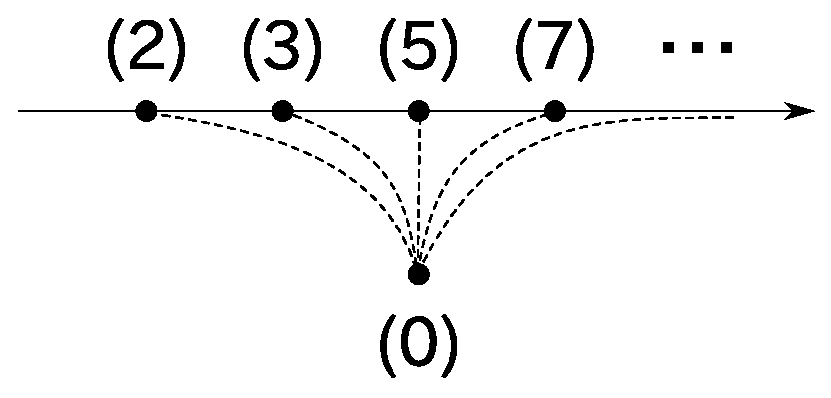
\includegraphics[width=5cm]{./images/SpecZ.eps}
    \end{center}
    \end{figure}

    任意の環$R$について,homomorphism $\phi: \Z \to R$を考える.
    準同型だから$\phi(0)=o, \phi(1)=e, \phi(-1)=-e$(ただし$o, e$はそれぞれ$R$の加法/乗法単位元.)となる.
    そして$\Z$は無限巡回群だから,$\phi(n-m)=\sum_{i=1}^n e+\sum_{i=1}^{m} (-e)$となり,
    よって準同型$\Z \to R$はただひとつ.
    つまり$|\Hom(\Z, R)|=1$.
    $\Spec \Z$はaffine spaceだから,Ex2.4より,任意のscheme $X$について$|\Hom(X, \Spec \Z)|=1$.
    すなわち,$\Spec \Z$は$\Sch$のfinal objectとなる.

\section{$\Spec \{0\}$ is the Initial Object in $\Sch$.} %% Ex2.6 
    零環$\{0\}$はただひとつのイデアル(したがって素イデアル)$(0)$を持つから,$\Spec \{0\}$は1点集合.
    零環から別の環への準同型写像は$0 \mapsto 0$なるものしか無い.
    schemeの間の射は環の間の準同型から作られるものしかないから(Prop2.3c),
    $\Spec \{0\}$から別のschemeへの射は$0 \mapsto 0$から得られるものしか無い.
    よって$\Spec \{0\}$はinitial object.

\section{Residue Field.} %% Ex2.7 
    Residue field of $x$ on $X$とは,剰余体$k(x):=\shO_{X,x}/\I{m}_{X,x}$のことである.

    $K$ :: field, $O:=(0) \subset K$とする.
    すると$\Spec K=\{O\}$であり,開集合は$\emptyset, \Spec K=\{O\}$の二つのみ.
    したがって$\shO_{\Spec K, O}=\shO_{\Spec K}(\Spec K)=K$となる.
    $\shO_{\Spec K, O}$は$\shO_{\Spec K}(\Spec K)$のみからなるdirect systemのdirect limitだから,
    これらは厳密に等しい.
    
    \paragraph{$(f,f^{\#}) \to (x, \phi)$}
    $(f, f^{\#}): (\Spec K, \shO_{\Spec K}) \to (X, \shO_X)$を考えよう.
    $f: \Spec K \to X$は,$\Spec K$が1点空間であることから,$f(O)$の値のみで定まる.
    この値を$x:=f(O)$としておこう.
    $f_* \shO_{\Spec K}$は
    \[
        f_* \shO_{\Spec K}(U)=
        \begin{cases}{}
            K & (x \in U) \\
            0 & (x \not \in U)
        \end{cases}
    \]
    で定まる.
    これは$K$のskyscraper sheaf (Ex.1.17)である.
    すると,$f^{\#}: \shO_X \to f_* \shO_{\Spec K}$は$x$におけるstalkの間の射
    \[ f^{\#}_{x}: \shO_{X,x} \to (f_* \shO_{\Spec K})_x=\shO_{\Spec K,O}=K \]
    を誘導する
    \footnote
        {
            この写像は$\varinjlim_{x \in U}f^{\#}$ではない.
            また,$(f_* \shO_{\Spec K})_x=\varinjlim_{x \in V \subseteq X} \shO_{\Spec K}(f^{-1}(V))=K.$
        }.
    これは以下の図式を可換にする射である.
    \[
    \xymatrix@C=5em
    {
    \shO_{X,x} \ar[r]^-{f^{\#}_{x}} & \shO_{\Spec K,O} \\
    \shO_X(U) \ar[r]^-{f^{\#}_U} \ar[u]_-{\mu_U} & \shO_{\Spec K}(\{O\}) \ar@{=}[u]
    }
    \]
    ただしこの図式では$x \in U \subseteq X$.
    今扱っているのはlocally ringed spaceのmorphismだから,
    \[ (f^{\#}_{x})^{-1}(\I{m}_{\Spec K,O})=(f^{\#}_{x})^{-1}(0)=\I{m}_{X,x}. \]
    よって$\ker f^{\#}_{x}=\I{m}_{X,x}$で,$(f^{\#})_{x}$は
    \[ \xymatrix{ \shO_{X,x} \ar@{->>}[r]& \shO_{X,x}/\I{m}_{X,x}=k(x)~ \ar@{>->}[r]^-{\phi} & K } \]
    へと分解される.
    こうして$(f,f^{\#})$から$x \in X$と$\phi_f: k(x) \to K$が得られた.

    \paragraph{$(x, \phi) \to (f,f^{\#})$}
    逆に$x \in X$と$\phi: k(x) \to K$から$(f,f^{\#})$を作る.
    これには以上の手順を逆にたどればよい.
    まず$f$は以下のものになる.
    \begin{defmap}
        f:& \Spec K& \to& X \\ 
        {}& O& \mapsto& x
    \end{defmap}
    $\phi: k(x) \to K$から$f^{\#}$を復元するには,以下のようにする.
    \begin{defmap}
        f^{\#}_U:& \shO_X(U)& \to& (f_* \shO_{\Spec K})(U) \\ 
        {}& s& \mapsto&
        \begin{cases}{}
            \Phi_U(s) & (x \in U) \\
            0 & (x \not \in U)
        \end{cases}
    \end{defmap}
    ここでの$\Phi_U ~(\text{with }x \in U)$は,以下のような写像の結合である.
    \[
        \xymatrix
        {
            \shO_X(U) \ar[r]
            & \varinjlim_{x \in V} \shO_X(V)=\shO_{X,x} \ar@{->>}[r]
            & \shO_{X,x}/\I{m}_{X,x}=k(x) \ar[r]^-{\phi}
            & K=(f_* \shO_{\Spec K})(U)
        }
    \]
    $f^{\#}$から$\phi$を作った時,$\phi$から再び$f^{\#}$に戻ることは,
    前段落で見た二つの図式から分かる.

\section{$\Hom_{/\Spec k}(\Spec k[x]/(x^2), X) \cong \Rat(X) \times T_x X$.} %% Ex2.8 
    $\epsilon=x+(x^2), D=k[x]/(x^2)=k[\epsilon]$とおく.
    $\epsilon^2=0$をよく使う.
    $(f, f^{\#}) \in \Hom_{/\Spec k}(\Spec D, X)$をとる.
    これは$\Spec k$上のmorphismである(教科書p.78参照).
    したがって
    \[ (p,p^{\#}): \Spec D \to \Spec k, (q,q^{\#}): X \to \Spec k \]
    が存在し$(p,p^{\#})=(q,q^{\#}) \circ (f, f^{\#})$が成立する.

    $O:=(0) \subset k, \I{m}:=\Nil(A)=(\epsilon)$とすると,
    Ex2.3bより$\Spec D \homeo \Spec D_{red}=\Spec k$.
    そこで$x=f(\I{m})$としておく.

    多項式環$k[x]$を$k$代数とみなすときは,
    自然な埋め込み射で$k$代数とみなす.
    \textbf{他の場合を考えることはない.}

    \paragraph{stalk間の写像.}
    特にstructure sheafの間に次の可換図式がある.
    \[
    \xymatrix@C=1em
    {
    p_* \shO_{\Spec D} & {} & \ar[ll]_-{q_*f^{\#}} q_* \shO_X \\
    {} & \ar[ul]^-{p^{\#}} \shO_{\Spec k} \ar[ur]_-{q^{\#}}& {}
    }
    \]
    この図式の射達から誘導される射達を書くと以下のようになる.
    (TODO: これは可換?)
    \[
    \xymatrix@C=1em
    {
    D=\shO_{\Spec D,\I{m}} & {} & \ar[ll]_-{f^{\#}_{\I{m}}} \shO_{X,x} \\
    {} & \ar[ul]^-{p^{\#}_{\I{m}}} k \ar[ur]_-{q^{\#}_x}& {}
    }
    \eqno(dg2.18)
    \]
    この図式を図式$(dg2.18)$と呼ぶことにする.
    ここで
    \[ \shO_{\Spec k,p(\I{m})}=\shO_{\Spec k,qf(\I{m})}=\shO_{\Spec k,O}=k,~~ \shO_{\Spec D,\I{m}}=D_{\I{m}}=D \]
    を用いた
    \footnote
        {
            $\frac{a+b\epsilon}{c+d\epsilon} \in D_{\I{m}}$は(分母) $ \not \in (\epsilon)$なので$c \neq 0$.
            分子分母に$c-d\epsilon$をかけると$\frac{ac+(bc-ad)\epsilon}{c^2}$となり,$D_{\I{m}}=D$が示される.
        }
    .

    \paragraph{$k \cong k(x)$.}
    図式$(dg2.18)$の射はいずれもlocal homomorphismだから,以下が成り立つ.
    \[ (p^{\#}_{\I{m}})^{-1}(\I{m})=(0),~~(q^{\#}_x)^{-1}(\I{m}_{X,x})=(0),~~(f^{\#}_{\I{m}})^{-1}(\I{m})=\I{m}_{X,x}  \]
    $ev_0$を$\epsilon \mapsto 0$という代入写像だとすると,これは全射.
    $ev_0^{-1}(0)=\I{m}, (f^{\#}_{\I{m}})^{-1}(\I{m})=\I{m}_{X,x}$より
    $\ker (ev_0 \circ f^{\#}_{\I{m}})=\I{m}_{X,x}$.
    なので準同型定理が使える.
    $\ker (ev_0 \circ p^{\#}_{\I{m}})^{-1}=(0)$も同様にして得られる.
    標準的全射$\shO_{X,x} \to k(x)$を用いれば$q^{\#}_x$についても同様である.
    \[
    \xymatrix@R=3em
    {
    k & {} & \ar@{>->}[ll] ~k(x) \\
    D \ar@{->>}[u]_-{ev_0} & {} & \ar[ll]_-{f^{\#}_{\I{m}}} \shO_{X,x} \ar@{->>}[u] \\
    {} & \ar[ul]^-{p^{\#}_{\I{m}}} k \ar[ur]_-{q^{\#}_x}& {}
    }
    \]
    $p^{\#}$は標準的入射であり,したがって$p^{\#}_{\I{m}}|_{k}=\id[k]$となっている.
    なので図式にある$k \to k$の射は全単射であり,
    このことと図式の可換性から$k \cong k(x)$が分かる
    ($g \circ f$が全射ならば$g$も全射であることを使う).

    \paragraph{$(f,f^{\#})$から$v_f \in T_x X$を構成する.}
    $\I{m} \subseteq f^{\#}_{\I{m}}(\I{m}_{X,x})$であるから,以下が成り立つ.
    \[
        \Forall{a \in \I{m}_{X,x} \subset \shO_{X,x}} \Exists{\beta \in k}
        f_{\I{m}}^{\#}(a)=\beta \epsilon \in \I{m}=(\epsilon).
    \]
    $aa' \in \I{m}_{X,x}^2$については$\epsilon^2=0$より$f_{\I{m}}^{\#}(aa')=0$となる.
    よって$\I{m}_{X,x}^2 \subseteq \ker f_{\I{m}}^{\#}$が得られる.
    なので
    \[ T_x X \ni v_f=\frac{1}{\epsilon}f_{\I{m}}^{\#}: \I{m}_{X,x}/\I{m}_{X,x}^2 \to k \]
    が得られる.

    \paragraph{$x \in \Rat(X), v \in T_x X$から$(f_v,f_v^{\#})$を構成する.}
    $\Spec D=\{\I{m}\}$なので$f_v: \I{m} \mapsto x$とする.
    $k(x)=k$だから,$a \mapsto a(x)$なる代入写像
    (これは$a \mapsto a \bmod \I{m}_{X,x}$と見ても同じ)は$k$に値を取る.
    また,$a-a(x)$は同じ代入写像で0になるから$\I{m}_{X,x}$に属す.
    そこで$a \in \shO_{X,x}$に対し,以下のように定める.
    \[ (f_v^{\#})_x(a)=a(x)+v([a-a(x)] \bmod \I{m}_{X,x}^2)\epsilon. \]
    さらに$U \subset X$について
    \[
        ((f_v)_* \shO_{\Spec D})(U)
        =\shO_{\Spec D}(f_v^{-1}(\{x\} \cap U))
        =
        \begin{cases}{}
            D_{\I{m}}=D & (x \in U) \\
            0   & (x \not \in U)
        \end{cases}
    \]
    だから,$x \in V \subseteq X$について以下の可換図式が得られる.
    \[
    \xymatrix
    {
    \shO_{X,x} \ar[r]^-{(f_v^{\#})_x} & D \\
    \shO_{X}(V) \ar[r]_-{(f_v^{\#})_V} \ar[u]& D \ar@{=}[u]
    }
    \]
    $x \not \in V$については,
    $((f_v)_* \shO_{\Spec D})(V)=0$なので$(f_v^{\#})_V$が自動的に零写像になる.
    こうして$f_v^{\#}$が構成できた.

    \paragraph{1対1対応であること.}
    容易に確かめられるので省略.

\section{Uniquely-Existence of Generic Point.} %% Ex2.9 
    $X$をschemeとし,$Z$をそのnonempty irreducible closed subsetとする.
    この時,$Z$がただひとつのgeneric pointを持つことを示す.

    \paragraph{Affine Case.}
    affine scheme $\Spec A$のirreducible closed subset $C$を考えよう.
    これは$\{ \I{p} \in \Spec A \mid \I{a} \subseteq \I{p} \}$のように表される
    素イデアルの集合である.
    Ati-Mac Exc1.8
    \footnote
    {
        これは以下のように解く.
        $C$の全順序部分集合$\Gamma$を考え,$\gamma=\bigcap \Gamma$とする.
        $\gamma \in C$を示せば良い.非自明な部分は$\gamma \in \Spec A$のみ.
        $x, y \in A$について$x, y \not \in \gamma$であったと仮定しよう.
        すると$x \not \in \I{p}, y \not \in \I{q}$となる$\I{p}, \I{q} \in \Gamma$が存在する.
        $\Gamma$は全順序なので,$\I{p} \subseteq \I{q}$と仮定できる.
        すると$x,y \not \in \I{p}$.
        $\I{p}$は素イデアルなので$xy \not \in \I{p}$が得られる.
        よって$x, y \not \in \gamma$ならば$xy \not \in \gamma$.
    }
    から,$C$は包含関係に関しての極小元を持つ.
    この極小元全体を$G$とおくと,これは1点からなる.
    これを示すため,$G$が2点以上からなると仮定しよう.
    すると$G$は空でない二つの真の部分集合の和$G=G_0 \cup G_1$として書くことが出来る.
    すると$G, G_0, G_1$の定義から
    \[ \cl_C(G_0), \cl_C(G_1) \subsetneq C \mand \cl_C(G)=C. \]
    閉包に関するgeneral topologyの結果から
    \[ C=\cl_C(G)=\cl_C(G_0 \cup G_1)=\cl_C(G_0) \cup \cl_C(G_1)=C. \]
    こうして$C$は空でない真の閉部分集合の和で書けることがわかった.
    これは$C$はirreducibleであることに反する.
    よって背理法により$G$が1点集合であることがわかった.
    これは$C$がただ1つのgeneric pointを持つことを意味する.

    \paragraph{Useful Fact (!).}
    一般に,$D \subset X$が$X$のdense subsetならば,
    $X \setminus D$は空集合の他に開集合を含まない.
    これは直ちに理解できるが重要なので記しておく.

    \paragraph{General Case.}
    affine open subset $U \subseteq X$であって,
    $U \cap Z \neq \emptyset$であるものをとる.
    この時,$U \cap Z$ ( :: closed in $U$)はaffine schemeのclosed subsetだから,
    前段落より,必ずgeneric point $\zeta$を持つ.
    この$\zeta$は$Z$のgeneric pointでもある.
    このことを示すために,$\{\zeta\}$が$Z$でdenseでないとしよう.
    すると$Z \setminus \{\zeta\}$は$V (\neq \emptyset)$ :: open in $Z$を含む.
    $Z$はirreducibleだから$V \cap U \neq \emptyset$.
    今$\zeta$は$Z \cap U$のgeneric pointとしたから,
    $(U \cap Z) \setminus \{\zeta\}=U \cap (Z \setminus \{\zeta\})$は
    $U \cap Z$の開集合を含まない.
    しかし今
    \[
        V \subseteq Z \setminus \{\zeta\}
        \text{ であり, }
        \emptyset \neq U \cap V \subseteq U \cap (Z \setminus \{\zeta\}).
    \]
    これは$\zeta$が$U \cap Z$のgeneric pointで無いことを意味し,$\zeta$のとり方に反する.
    よって$\zeta \in U \cap Z$は$Z$のgeneric pointである.
    また,$\zeta$の他にgeneric point $\zeta'$が存在したとしよう.
    $\zeta' \not \in Z \cap U$であれば$Z \setminus \{\zeta'\}$は
    空でない開集合$Z \cap U$を含むことになるので,$\zeta, \zeta' \in Z \cap U$.
    前段落の結果より,$\zeta=\zeta'$が得られる.

\section{$\Spec \R[x]$} %% Ex2.10 
    $\Spec \R[x]$の元は,既約多項式または0が生成する単項イデアルである.
    $\R[x]$の既約多項式は,一次式または二次式に限られる(代数学の基本定理の初期バージョン).
    したがって$\R[x]$の既約多項式は
    \[ \C_{\Im \geq 0}=\{ x+iy \mid y \geq 0 \} \]
    の元と一対一に対応する.

\section{$\Spec \mathbb{F}_p[x]$} %% Ex2.11 
    図を書くと次のようになる.
    \begin{figure}[ht]
    \begin{center}
        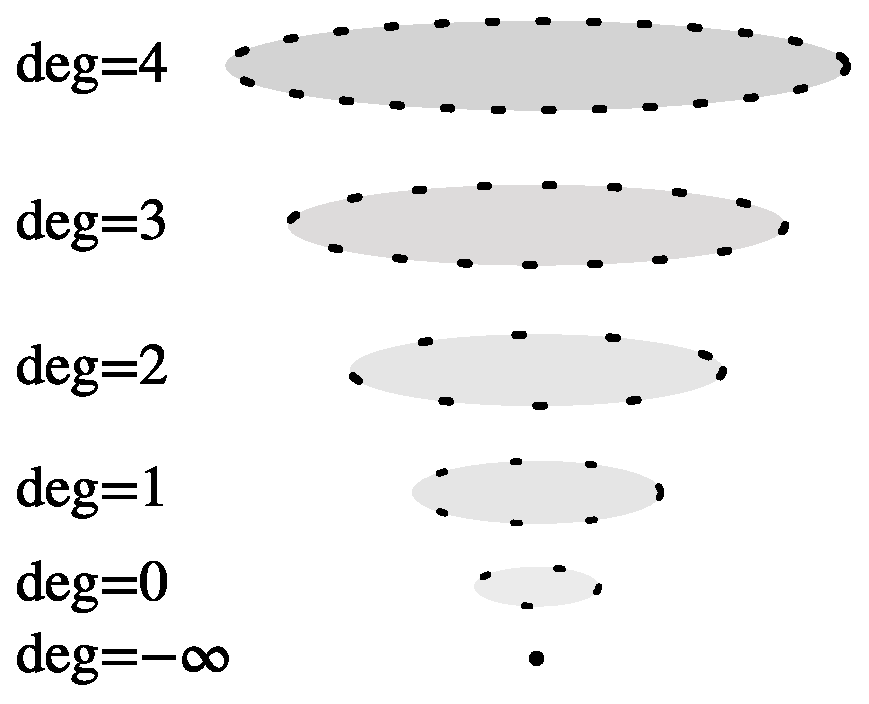
\includegraphics[width=5cm]{./images/SpecF_p[x].eps}
    \end{center}
    \end{figure}
    この円錐は上へ限りなく続く.

\section{Gluing Lemma.} %% Ex2.12
    データは次の通り.
    \begin{itemize}
        \item $\{U_i\}_{i \in I}$ :: family of schemes,
        \item $\{U_{ij}\}_{i,j \in I}$ :: open subschemes ($U_{ij} \subset X_i$), and
        \item $\{\phi_{ji}:U_{ij} \to U_{ji}\}_{i,j \in I}$ :: isomorphisms of schemes.
    \end{itemize}
    $\phi_{ji}$の添字の順番がHartshorneの逆なので注意.
    これらは次を満たす:
    \begin{enumerate}[label=(\arabic*)]
        \item $\Forall{i \in I} U_{ii}=U_i$.
        \item $\Forall{i,j,k \in I} \phi_{kj} \circ \phi_{ji}=\phi_{ki}$ ~on~ $U_{ij} \cap U_{ik}$.
    \end{enumerate}
    $\#I=3$の場合の図は次の様になる.
    \begin{figure}[ht]
    \begin{center}
        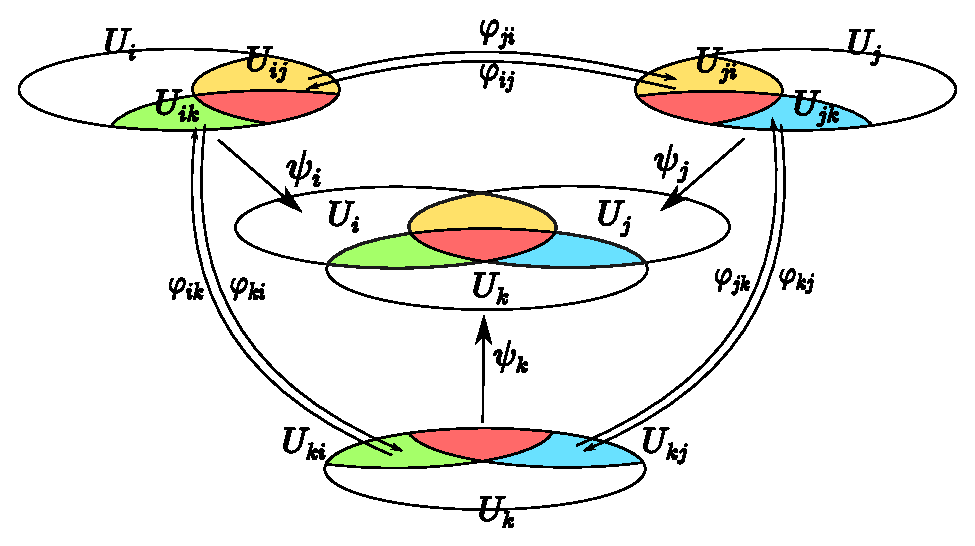
\includegraphics[width=8cm]{./images/gluing.eps}
    \end{center}
    \end{figure}

    1つめの条件から$\phi_{ii}=\id[U_{ii}]$が従う.
    2つめの条件はcocycle conditionと呼ばれる.
    この条件で$i=k$とすれば$\phi_{ij}=\phi_{ji}^{-1}$が分かる.
    $\phi_{ij}(U_{ij} \cap U_{ik})=U_{ji} \cap U_{jk}$も同様.
    これを図にすれば次のようになる.
    \begin{figure}[ht]
    \begin{center}
        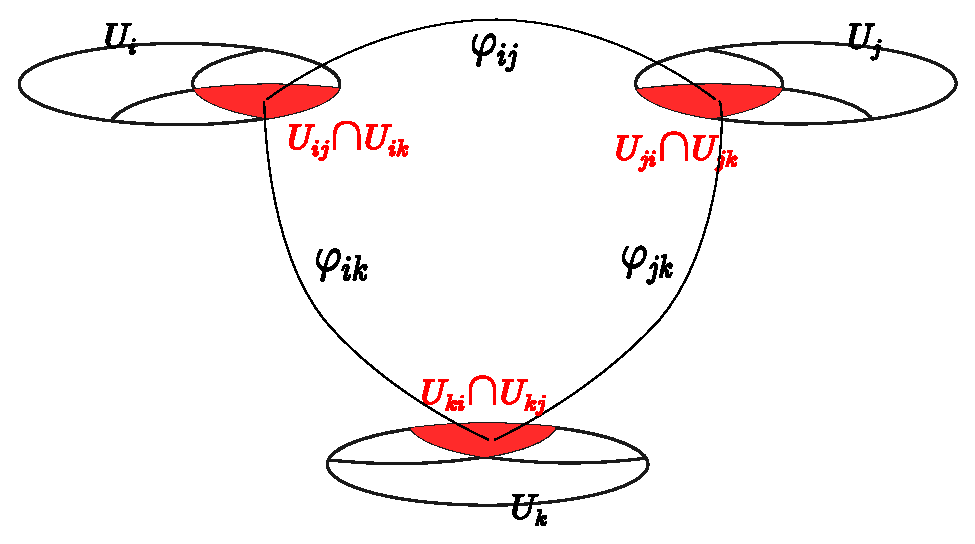
\includegraphics[width=8cm]{./images/cocycle_cond.eps}
    \end{center}
    \end{figure}

    これらのデータから得られるcolimitが$\{U_i\}_{i \in I}$のgluingである.
    すなわち,
    これらのデータから,次の性質を満たす
    $X$ :: schemeと$\{\psi_i: U_i \to X\}_{i \in I}$が得られる.
    \begin{itemize}
        \item $\im \psi_i$ :: open subscheme of $X$ (for all $i \in I$).
        \item $\psi_i: U_i \to \im \psi_i$ :: isomorphism (for all $i \in I$).
        \item $\psi_j \circ \phi_{ji}=\psi_i$ on $U_{ij}$ (for all $i,j \in I$).
        \item $X=\bigcup_{i \in I} \psi_i(U_i)$.
        \item $\psi_i(U_{ij})=\psi_i(U_i) \cap \psi_j(U_j)=\psi_j(U_{ji})$ (for all $i,j \in I$)
    \end{itemize}
    また,$X, \{\psi_i\}_i$は与えられたデータから同型を除いて一意に定まる.

    命題(colimitの存在)の証明の詳細は
    U.Gortz, T.Wedhorn ``Algebraic Geometry I"のpp.70-71を参照するのが良い.
    ここでは概要
%    と,``Algebraic Geometry I"で述べられていない詳細
    を述べる.

    まず,$\basesp X$は$\{ U_i \}_i$と$\{ \phi_{ij} \}_{i,j}$が成す
    index categoryのcolimitとして与えられる.
    すなわち,次のように与えられる.
    \[ \basesp X=\bigsqcup_{i \in I} U_i \Big/ \sim. \]
    ただし,$\sim$は次のような二項関係である.
    \[
        \Forall{i,j \in I}
        \Forall{x_i \in U_i, x_j \in U_j}
        \lbra{~ x_i \sim x_j \iff x_j=\phi_{ji}(x_i) ~}.
    \]
    この二項関係が同値関係であること,
    及びwell-definedであることは,cocycle conditionから得られる.
    これは商位相だから,$V \subseteq X$が開集合であることは
    すべての$i$について$\psi_i^{-1}(V)$が$U_i$の開集合であることと同値.
    特に,$\im \psi_i=\psi_i(U_i)$は
    $\psi_i^{-1}\psi_i(U_i)=U_i$ゆえに開集合である.

    次に,$\shO_X$は次の様に与えられる.
    こちらはlimitである.
    (schemeはtopologyとsheafで射が反転することによる.)
    $V$を$X$の開集合とする.
    \[
        \shO_X(V)=
        \left\{
            \Sigma \in \prod_{i \in I} \shO_{U_i}(\psi_i^{-1}V)
            ~\middle|~
            \Forall{i,j \in I}
            \phi^{\#}_{ij} \left( \Sigma_j|_{\psi_j^{-1}V \cap U_{ji}} \right)=\phi^{\#}_{ii} \left( \Sigma_i|_{\psi_i^{-1}V \cap U_{ij}} \right)
        \right\}.
    \]
    $\Sigma$の$i$成分を$\Sigma_i (\in \shO_{U_i}(\psi_i^{-1}V))$と書いている.
    $\phi_{ii}=\id[U_{ii}]=\id[U_i]$に注意.
    これはinverse limitなので,Ex1.12より,これもsheaf.

\section{Quasi-Compact/Noetherian Space.} %% Ex2.13 
    \begin{Lemma}[I]
        $A$ :: ring, $f \in A$について$D(f)$ :: quasi-compact.
    \end{Lemma}
    \begin{proof}
        $D(f)=\bigcup_{i \in I} U_i$とすると,
        \[ \sqrt{(f)}=\sqrt{\sum_{i \in I} \I{a}_i} \]
        というイデアル達$\{\I{a}_i\}_{i \in I}$が存在する.
        両辺ともに特に$f$を含むから,ある自然数$n>0$が存在して
        \[ f^n \in \sum_{i \in I} \I{a}_i \]
        となる.
        イデアルの和の定義から,(必要なら適当に番号を付け替えることで)
        \[ f^n=\sum_{i=1}^{r} a_i \text{ with } a_i \in \I{a}_i \]
        と出来る.
        よって
        \[
            \sqrt{(f)}
            \subseteq \sqrt{\sum_{i=1}^{r} \I{a}_i}
            \subseteq \sqrt{\sum_{i \in I} \I{a}_i}=\sqrt{(f)}
        \]
        となる.
        これは$D(f)=\bigcup_{i=1}^r U_i$を意味する.
    \end{proof}
    \begin{Lemma}[II]
        $V(\I{a})^c$ :: quasi-compact
        $\iff$
        $\sqrt{\I{a}_f}=\sqrt{\I{a}}$となる有限生成イデアル$\I{a}_f$が存在する.
    \end{Lemma}
    \begin{proof}
        \paragraph{($\implies$).}
        $\I{a}=\sum_{a \in A} (a)$だから
        \[ V(\I{a})^c=V(\sum_{a \in A} (a))^c=\bigcup_{a \in A} V((a))^c \]となる.
        仮定より
        \[ V(\I{a})=V(\sum_{i=1}^r (a_i))^c=V(\langle a_1,\dots,a_r\rangle) \]
        となる$a_i \in \I{a}$が存在する.

        \paragraph{($\impliedby$).}
        $g_1,\dots,g_r$を$\I{a}_f$の生成元とすると
        \[ V(\I{a})^c=V(\sum_{i=1}^r (g_i))^c=\bigcup_{i=1}^r D(g_i) \]となる.
        これはLemma Iよりquasi-compactな開集合の有限和だから,quasi-compact.
    \end{proof}

    \subsection{Noethrian $\iff$ Every Open Subset is Quasi-Compact.}
    \paragraph{($\implies$).}
    Ch.I, Ex1.7ですべて示した.

    \paragraph{($\impliedby$).}
    可算開集合族$\mathfrak{U}=\{U_i\}_{i \in \N}$が昇鎖$U_0 \subseteq U_1 \subseteq \dots$をなすとしよう.
    $U=\bigcup_{i \in \N} U_i$とすると,$\mathfrak{U}$は$U$のopen coverである.
    なので仮定よりfinite sub-cover $\mathfrak{U}_{fin}$が存在する.
    $\mathfrak{U}$は昇鎖なので,$\mathfrak{U}_{fin}$も有限昇鎖をなす.
    その有限昇鎖の中でもっとも大きい物をとれば,それは$U$と一致する.
    これで主張が示せた.

    \subsection{$\Spec A$ :: Quasi-Compact, but NOT Noetherian In General.}
    $X=\Spec A$とする.
    $D(1)=\Spec A$だから,Lemma Iより$\Spec A$ :: quasi-compact.
    しかし一般にはNoetherianでない.
    これを示すためには,(a)から,ある開集合がquasi-compactでない例を構成すれば良い.
    そのために
    \[ A=k[x_1,x_2,\dots] \supset \I{a}=(x_1,x_2,\dots) \]
    を考える.ただし$k$ :: alg.closed.field.
    Lemma IIより,
    $\sqrt{\I{a}}=\sqrt{\I{a}_f}$となる有限生成イデアル$\I{a}_f$が
    存在しないことを示せば良い.

    背理法で証明する.
    $\I{a}_f$が存在すると仮定し,$g_1,\dots,g_r$を$\I{a}_f$の生成元とする.
    各$g_i$に入っている不定元は高々有限個だから,
    まとめれば,$g_1,\dots,g_r$のいずれかに入っている不定元であって一番番号が大きいものが存在する.
    それを$x_N$としよう.つまり$g_1,\dots,g_r \in A_N$.
    $\I{a}_f^c=\I{a} \cap A_N$とおこう.

    $1 \in \I{a}_f^c \implies 1 \in \I{a}_f$だから,
    これの対偶によって$\zerosa(\I{a}_f^c) \neq \emptyset$(ここで$k$ :: alg.closedを使っている).
    \[ (\alpha_1,\dots,\alpha_N) \in \zerosa(\I{a}_f^c), P=(\alpha_1,\dots,\alpha_N,1,0,\dots) \]
    とすると,$g_i(P)=0$.
    一方,$x_{N+1} \in \sqrt{\I{a}}=\sqrt{\I{a}_f}$だから,
    $x_{N+1}^d=c_1g_1+\dots+c_Ng_N$となる$d>0$が存在する.
    両辺に$P$を代入すると,左辺は$1^d=1 \neq 0$.右辺は$c_1(P)*0+c_N(P)*0=0$.
    矛盾が生じた.
    よって$\sqrt{\I{a}}=\sqrt{\I{a}_f}$となる有限生成イデアル$\I{a}_f$は存在しない.

    \subsection{$A$ :: Noethrian $\implies$ $\Spec A$ :: Noethrian.}
    Lemma IIと(a)により明らか.

    \subsection{Give Example: $A$ :: Noetherian $\not \impliedby$ $\Spec A$ :: Noethrian.}
    $k$を体,$x_1,x_2,\dots$を不定元とし,$A=k[x_1,x_2,\dots]/(x_1,x_2,\dots)^2$を考える.
    $x_i$の$R$における像を$e_i$とすると,任意の$i,j$について$e_i e_j=0$.
    イデアル$(e_1,e_2,\dots)$は有限生成でないから,この環はNoetherian ringでない.
    $\Spec A$がNoetherianであることは,Ex2.3bと$\Nil(A)=(e_1,e_2,\dots)$から得られる.
    $\Nil(A)$は$e_i \mapsto 1$という代入写像の核だから極大イデアル.
    したがってEx2.3bより$\Spec A_{red} \homeo \Spec k$となり,
    これは1点集合である.
    よってNoetherian.

\section{$\Proj S$} %% Ex2.14 

\section{The Fuctor $t$.} %% Ex2.15 

\section{$X_f$.} %% Ex2.16 
    $X$ :: scheme, $f \in \Gamma(X, \shO_X)=:A$について,
    $X_f$を次のように定める.
    \[ x \in X_f \iff f_x \text{ :: unit in }\shO_{X,x}. \]

    \subsection{For $X \supseteq U=\Spec B$, $X_f \cap U=D(\bar{f}).$}
    $U \subseteq X$をopen affine subschemeとし,$U=\Spec B$とする.
    さらに$\bar{f}$で$f|_{U} \in \Gamma(U,\shO_X|_U)=B$を表す.
    この時,以下が成り立つ.
    \begin{align*}
        {}&     x \in X_f \cap U \\
        \iff&   [ f_x \text{ :: unit in }\shO_{X,x}] \land [x \in U] \\
        \iff&   \bar{f}_x=\frac{\bar{f}}{1} \text{ :: unit in }B_{\I{p}_x} \\
        \iff&   \bar{f} \not\in \I{p}_x \\
        \iff&   x \in D(\bar{f})
    \end{align*}
    ただし$\I{p}_x \subseteq B$は点$x$に対応する素イデアル.
    よって$X_f \cap U=D(\bar{f})$.

    $U$ :: open in $X$かつ$X_f \cap U=D(\bar{f})$ :: open in $U$なので,
    $X_f \cap U$ :: in $X$.
    $X$のopen affine coverを考えれば,$X_f$ :: open in $X$が分かる.

    \subsection{For $a \in A$,If $X$ :: quasi-compact and $a|_{X_f}=0$ then $\Exists{n > 0} f^n a=0$.}
    $\{U_i\}_{i \in I}$を$X$のopen affine coverとする.
    $X$ :: quasi-compactという仮定から,$I$は有限であると仮定して構わない.
    また,$U_i = \Spec B_i$とする.

    $a \in A$をとり,$a|_{X_f}=0$であるとする.
    すると任意の$i$について$a|_{U_i}=0(=0/1)$,$a|_{U_i} \in B_i$.
    前sectionから$X_f \cap U=D(f|_{U_i})$なので,以下が成り立つ
    \footnote{商環の等号の定義からは$n_i \geq 0$であるが,$n_i>0$としても問題ない.}.
    \[ \Forall{i \in I} \Exists{n_i>0} (f|_{U_i})^{n_i}(a|_{U_i} \cdot 1-1 \cdot 0)=(f^{n_i}a)|_{U_i}=0. \]
    $I$は有限だから,$n=\max_{i \in I} n_i$が存在する.
    明らかに任意の$i$について$(f^{n}a)|_{U_i}=0$だから,
    Identity Axiomにより$f^n a=0$ in $A$.

    \subsection{Under Some Assumption, $\Forall{b \in \Gamma(X_f, \shO_{X_f})} \Exists{n>0} \Exists{a \in A} f^n b=a|_{X_f}$.}
    $X$はfinite affine open cover $\{U_i\}_{i=1}^r$を持ち,
    任意の$i,j$について$U_i \cap U_j$ :: quasi-compactであるとする.
    $U_i=\Spec B_i$とする.
    (次の問題(d)でも$X$にこの仮定を置く)

    (a)より$U_i \cap X_f=D(f|_{U_i})$,かつProp2.2より$\shO_{U_i}(D(f|_{U_i}))=(B_i)_{f|_{U_i}}$.
    なので$b|_{D(f|_{U_i})} \in (B_i)_{f|_{U_i}}$について以下が成り立つ.
    ただし$f_i=f|_{U_i}$とした.
    \[ \Exists{m_i>0} \Exists{b_i \in B_i} (f^{m_i}b)|_{D(f_i)}=b_i|_{D(f_i)}. \]
    $m=\max_i m_i$とすれば以下のようにまとめられる.
    \[ \Exists{a_i \in B_i} (f^{m}b)|_{D(f_i)}=a_i|_{D(f_i)}. \]

    次に$a_i \in B_i=\Gamma(U_i, \shO_{U_i})$を貼りあわせる.
    そのために(b)を,$X=U_i \cap U_i$として利用しよう.
    $X_{ij}=U_i \cap U_j, f_{ij}=f|_{U_i \cap U_j} \in \Gamma(U_{ij},\shO_{U_{ij}})$とおく.
    すると$(X_{ij})_{f_{ij}}=X_f \cap X_{ij}$となる.
    $a_i-a_j \in \Gamma(U_{ij},\shO_{U_ij})$を$(X_{ij})_{f_{ij}} \subset D(f_{i})$に制限すると0になるから,
    (b)より,以下が成り立つ.
    \[ \Exists{n_{ij}>0} (f_{ij})^{n_{ij}}(a_i-a_j)=0. \]
    これをすべての組$(i,j)$について考えれば,以下が得られる.
    \[ \Exists{n>0} (f^n a_i)|_{U_{ij}}=(f^n a_j)|_{U_{ij}} \text{ in } \Gamma(U_{ij},\shO_{U_ij}).  \]
    よってGluability Axiomにより,$(f^n a)|_{U_i}=f^n a_i$となる$a \in A$がある.

    もとの$f^m b$へ戻ると,今以下が成り立つ.
    \[ (f^{m+n} b)|_{D(f_i)}=(f^n a)|_{D(f_i)}. \]
    Identity Axiomにより,$f^{m+n} b=(f^n a)|_{X_f}$.

    \subsection{$\Gamma(X_f, \shO_{X_f})=A_{f}$.}
    (c)から,以下が成り立つ.
    \[ \Forall{b \in \Gamma(X_f, \shO_{X_f})} \Exists{a \in A} \Exists{n>0} b=\frac{a}{f^n}. \]
    よって$\Gamma(X_f, \shO_{X_f}) \subseteq A_f$.
    $\supseteq$は明らかなので,$\Gamma(X_f, \shO_{X_f}) \subseteq A_f$.

\section{A Criterion for Affineness.} %% Ex2.17 
    \subsection{$f|_{f^{-1}(U_i)}$ :: iso $\implies$ $f$ :: iso.}
    $f: X \to Y$ :: morphism of schemesについて,
    open cover $\{U_i\}$が存在し,
    各$i$について$f_i:=f|_{f^{U_i}}: f^{-1}(U_i) \to U_i$がisoであったとする.
    この時$f$ :: isoを示す.
    $V_i=\{f^{-1}(U_i)\}$としておく.これは$X$を被覆する.

    \[ f_i|_{V_i \cap V_j}=(f|_{V_i})|_{V_i \cap V_j}=(f|_{V_j})|_{V_i \cap V_j}=f_i|_{V_i \cap V_j} \]
    なので,$f$は$f_i$達の張り合わせとして矛盾なく書くことが出来る.
    つまり,「$f(x)=f_i(x)$(ここでの$i$は$x \in V_i$を満たすもの)」と書くことが出来る.
    さらに$V,U$ :: open in $X, Y$について,以下が成り立つ.
    \[ f(V)=f(\bigcup (V \cap V_i))=\bigcup f(V \cap V_i);~~ f^{-1}(U)=f^{-1}(\bigcup (U \cap U_i))=\bigcup f^{-1}(U \cap U_i). \]
    $f_i$:: homeoからこの二つは開集合.
    よって$f$ :: homeo.

    $f^{\#}: \shO_{Y} \to f_* \shO_{X}$も次のように$f_i^{\#}$で書ける.
    \[
        \shO_{Y}(U) \to f_* \shO_{Y}(U):
        \xymatrix{
        s \ar@{|->}[r]
        & \bigoplus (s|_{U \cap U_i}) \ar@{|->}[rr]^-{\bigoplus (f_i^{\#})_{U \cap U_i}}
        & {}
        & \bigoplus (f_i^{\#})_{U \cap U_i}(s|_{U \cap U_i})=\bigoplus t_i \ar@{|->}[r]
        & t
        }
    \]
    $(f_i^{\#})_{U \cap U_i}$がisoなのでこの写像はiso.

    \subsection{For scheme $X$, $X$ :: affine $\iff$ ....}
    $X$ :: schemeを考える.$A:=\Gamma(X, \shO_X)$とする.
    以下を条件(*)と呼ぶ.
    \[ \Exists{f_1, \dots, f_r \in A=\Gamma(X, \shO_X)} [\Forall{i=1,\dots,r} X_{f_i} \text{ :: affine}] \land [(f_1,\dots,f_r)=(1)=A.] \]
    $X$ :: affine $\iff$ (*),ということを示す.
    Affine schemeはquasi-compactである(Ex2.13b),ということを何度も使う.

    \paragraph{$\implies$.}
    この時$X=\Spec A$である.
    主張の成立は自明.

    \paragraph{$\impliedby$.}
    核心となるのは,$\{X_{f_i}\}$がEx2.16cで$\{U_i\}$に課せられている条件を満たす,ということ.
    $X=\bigcup X_{f_i}$は
    \[ \left( \bigcup X_{f_i} \right)^c=\left( \bigcap \{x \mid (f_i)_x \in \I{m}_{X,x} \subset \shO_{X,x}\} \right)^c \]
    と$(f_1,\dots,f_r)=(1)$から得られる.
    $X_{f_i} \cap X_{f_j}$ ::quasi-compactは,$X_{f_i}=\Spec F_i$とすると,
    \[ X_{f_i} \cap X_{f_j}=D(f_j|_{X_{f_i}})=\Spec (F_i)_{f_j} \]はaffine schemeだからquasi-compact.
    以上からEx2.16d, Ex2.4, Ex2.17aが全部使えて,この順に使えば$X=\Spec A$が示せる.

\section{Ring Homomorphism vs. the Induced Morphism of the Spectra.} %% Ex2.18 
    $A,B$ :: ring, $\phi: A \to B$ :: ring homoとする.
    $(f,f^{\#}): Y=\Spec B \to \Spec A=X$と$\phi$の関係を考える.
    以下では$f(y) \in X$における$f^{\#}$のstalkを$f^{\#}_{(y)}$と書く.

    \[
        \xymatrix
        {
        \shO_{X,f(y)} \ar[r]^{}f^{\#}_{(y)} & (f_* \shO_{Y})_{f(y)} \ar[r]^{\iota^y}& \shO_{Y,y} \\
        A_{f(y)} \ar@{<->}[u] \ar[rr]^{\phi_{y}} & {} & B_y \ar@{<->}[u]
        }
    \]


\section{$\Spec A$ :: disconnected $\iff$ ....} %% Ex2.19 
    可換環$A$について以下が同値であることを示す.
    \begin{enumerate}[label=(\arabic*)]
    \item $\Spec A$ :: disconnected.
    \item $\Exists{e_1, e_2 \in A \setminus \{0\}} e_1e_2=0, e_1^2=e_1, e_2^2=e_2, e_1+e_2=1$.
    \item $\Exists{A_1, A_2 \neq 0} A \cong A_1 \times A_2$.
    \end{enumerate}

    \paragraph{(1)$\implies$(2) [Step 1]}
    仮定より,$\Spec A$は二つ以上のconnected componentをもつ.
    そこで一方のconnected componentを$C_1$とし,$C_2=\Spec A \setminus C_1$とする.
    そして$\I{a}_1=\bigcap_{\I{p} \in C_1}$とし,$\I{a}_2$も同様に定義する.
    定義の仕方から,$\I{a}_1 \subsetneq \I{a}_1'$であるとき
    \[ C_1=V(\I{a}_1) \supsetneq V(\I{a}_1') \]
    となることに注意せよ.

    \paragraph{(1)$\implies$(2) [Step 2]}
    \begin{align*}
        {}& \Spec A=V(\I{a}_1) \sqcup V(\I{a}_2) \\
        \iff& [\Spec A=V(\I{a}_1 \I{a}_2)] \land [\emptyset=V(\I{a}_1+\I{a}_2)] \\
        \iff& [\I{a}_1 \I{a}_2 \subseteq \Nil(A)] \land [(1)=\I{a}_1+\I{a}_2] \label{ex219-1}
    \end{align*}
    最後の行,2つめの条件から,
    $a_1+a_2=1$となる$a_1 \in \I{a}_1, a_2 \in \I{a}_2$が存在することが分かる.
    1つめの条件からは,$a_1^n a_2^n=0$となる$n>0$が存在することが分かる.

    \paragraph{(1)$\implies$(2) [Step 3]}
    $(a_1+a_2)^n=1^n=1$の左辺を展開する.
    \[ 1=a_1^n+a_2^n+a_1a_2 \left( \sum_{i=1}^{n-1} \binom{n}{i}a_1^{i-1}a_2^{n-i-1} \right)=1. \]
    $a_1a_2(***)$の部分を移項すると,
    \[ a_1^n+a_2^n=1-a_1a_2(***) \]
    となる.
    $a_1a_2(***) \in \Nil(A)$だから,Ati-Mac Ex1.1より右辺は単元.
    これを$u$を置くと,
    \[ u^{-1}a_1^n+u^{-1}a_2^n=1, (u^{-1}a_1^n)(u^{-1}a_2^n)=u^{-2}(a_1^na_2^n)=0 \]
    となる.

    \paragraph{(1)$\implies$(2) [Step 4]}
    以上から,$e_1=u^{-1}a_1^n, e_2=u^{-1}a_2^n$とおくと
    $e_1+e_2=1$と$e_1e_2=0$が成り立つことがわかった.
    最後に,$e_1^2=e_1$を示す($e_1^2=e_1$も同様).
    これは以下のように直ちに示せる.
    \[ e_1 \cdot (e_1+e_2)=e_1 \cdot 1 \implies e_1^2+e_1e_2=e_1 \implies e_1^2=e_1. \]

    \paragraph{(2)$\implies$(3)}
    $A_1=e_1 A, A_2=e_2 A$とすれば良い.
    同型は以下のように定義できる.
    \begin{defmap}
        \phi:& A_1 \times A_2& \to& A \\ 
        {}& (x,y)& \mapsto& x+y \\
        {}& (a e_1,a e_2)& \mapedfrom& a
    \end{defmap}
    $a_1 \in A_1, a_2 \in A_2$について$a_1 a_2=0$に注意すると,
    準同型であることが確かめられる.
    実際,
    \[ \phi(x,y) \phi(z,w)=(x+y)(z+w)=xz+(yz+zw)+yw=xz+yw=\phi(xz,yw)=\phi((x,y)\cdot(z,w)). \]
    同型であることは$e_1+e_2$にも注意すれば分かる.

    \paragraph{(3)$\implies$(1)}
    $e_1,e_2$があるとき,$(e_1), (e_2)$は明らかに(\label{ex219-1})を満たす.
    なので$\Spec A=V((e_1)) \sqcup V((e_2))$となる.

\end{document}
